Uno de los trabajos más relevantes sobre la representación de una neurona biológica fue el de Warren McCulloch y Walter Pitts quienes se consideran  pioneros en el campo de las neurociencias computacionales y la teoría de las redes neuronales artificiales. En 1943, publicaron un artículo titulado ``A Logical Calculus of Ideas Immanent in Nervous Activity'' (``Un cálculo lógico de ideas inmanentes en la actividad nerviosa''), donde presentaron un modelo muy simplificado de una neurona biológica, que es considerado uno de los primeros modelos de neuronas artificiales\cite{mcculloch1943logical}.

\begin{figure}[h!]
	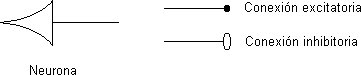
\includegraphics[width=0.65\textwidth]{capitulo2/figuras/an2.png}
	\caption[Representacion grafica de una neurona y sus dos tipos de conexiones]{Representacion grafica de una neurona y sus dos tipos de conexiones\\\textit{Fuente: Extraído de} \protect\cite[ p.4]{prieto2020modelo} }
	\label{fig:an2}
\end{figure}

Este modelo propuesto  fue una abstracción matemática de cómo funciona una neurona biológica, y fue formulado como un sistema de lógica binaria. En su modelo, una neurona recibe múltiples señales de entrada (excitatorias o inhibitorias) y produce una única salida binaria basada en una función umbral. Si la suma de las señales de entrada superaba un cierto umbral, la neurona se activaba y emitía una señal de salida, de lo contrario, permanecía inactiva.

\begin{figure}[h!]
	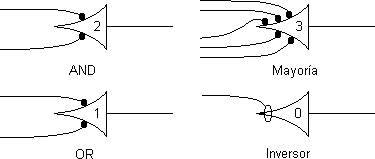
\includegraphics[width=0.65\textwidth]{capitulo2/figuras/an3.png}
	\caption[Algunos ejemplos de la implantacion de funciones logicas]{Algunos ejemplos de la implantacion de funciones logicas
		\\\textit{Fuente: Extraído de} \protect\cite[p. 5]{prieto2020modelo} }
	\label{fig:an3}
\end{figure}

Aunque este modelo es muy simple en comparación con la complejidad de las neuronas biológicas reales, sentó las bases para el desarrollo de redes neuronales artificiales, esto debido a que ellos podían darnos a entender que la resolución de problemas más complejos  podría ser posible con la  conexión de muchas de estas neuronas. En la Figura \ref{fig:an2} se puede observar la representación básica de una neurona interpretando al modelo de Warren McCulloch y Walter Pitts , donde se aborda y representa los conceptos de conexión excitatoria e inhibitoria, que es equivalente a la sinapsis excitatoria e inhibitoria de una neurona biológica. En la Figura \ref{fig:an3} en la esquina superior izquierda se puede observar a la representación de una neurona cuyo funcionamiento es equivalente a una compuerta and de dos entradas, en la esquina inferior izquierda se encuentra otra neurona que es equivalente a una compuerta or de dos entradas , en la esquina superior derecha se aprecia a una neurona or de 5 entradas con un umbral de tres y finalmente en la esquina inferior derecha se observa una neurona con una  conexión inhibitoria con umbral cero.





